% Тип документа
\documentclass[a4paper,12pt]{extarticle}

% Шрифты, кодировки, символьные таблицы, переносы
\usepackage{cmap}
\usepackage[T2A]{fontenc}
\usepackage[utf8x]{inputenc}
\usepackage[russian]{babel}

% Это пакет -- хитрый пакет, он нужен но не нужен
\usepackage[mode=buildnew]{standalone}

\usepackage
	{
		% Дополнения Американского математического общества (AMS)
		amssymb,
		amsfonts,
		amsmath,
		amsthm,
		physics,
		% misccorr,
		% 
		% Графики и рисунки
		wrapfig,
		graphicx,
		subcaption,
		float,
		tikz,
		tikz-3dplot,
		caption,
		csvsimple,
		color,
		booktabs,
		pgfplots,
		pgfplotstable,
		geometry,
		% 
		% Таблицы, списки
		array,
		makecell,
		multirow,
		indentfirst,
		%
		% Интегралы и прочие обозначения
		ulem,
		esint,
		esdiff,
		% 
		% Колонтитулы
		fancyhdr,
	}  

\usepackage{xcolor}
\usepackage{hyperref}

 % Цвета для гиперссылок
\definecolor{linkcolor}{HTML}{000000} % цвет ссылок
\definecolor{urlcolor}{HTML}{799B03} % цвет гиперссылок
 
\hypersetup{pdfstartview=FitH,  linkcolor=linkcolor,urlcolor=urlcolor, colorlinks=true}
% Обводка текста в TikZ
\usepackage[outline]{contour}

% Увеличенный межстрочный интервал, французские пробелы
\linespread{1.3} 
\frenchspacing 

 
\usetikzlibrary
	{
		decorations.pathreplacing,
		decorations.pathmorphing,
		patterns,
		calc,
		scopes,
		arrows,
		fadings,
		through,
		shapes.misc,
		arrows.meta,
		3d,
		quotes,
		angles,
		babel
	}


\tikzset{
	force/.style=	{
		>=latex,
		draw=blue,
		fill=blue,
				 	}, 
	%				 	
	axis/.style=	{
		densely dashed,
		blue,
		line width=1pt,
		font=\small,
					},
	%
	th/.style=	{
		line width=1pt},
	%
	acceleration/.style={
		>=open triangle 60,
		draw=magenta,
		fill=magenta,
					},
	%
	inforce/.style=	{
		force,
		double equal sign distance=2pt,
					},
	%
	interface/.style={
		pattern = north east lines, 
		draw    = none, 
		pattern color=gray!60,
					},
	cross/.style=	{
		cross out, 
		draw=black, 
		minimum size=2*(#1-\pgflinewidth), 
		inner sep=0pt, outer sep=0pt,
					},
	%
	cargo/.style=	{
		rectangle, 
		fill=black!70, 
		inner sep=2.5mm,
					},
	%
	caption/.style= {
		midway,
		fill=white!20, 
		opacity=0.9
					},
	%
	}

\newenvironment{tikzpict}
    {
	    \begin{figure}[htbp]
		\centering
		\begin{tikzpicture}
    }
    { 
		\end{tikzpicture}
		% \caption{caption}
		% \label{fig:label}
		\end{figure}
    }


\newcommand{\vbLabel}[3]{\draw ($(#1,#2)+(0,5pt)$) -- ($(#1,#2)-(0,5pt)$) node[below]{#3}}
\newcommand{\vaLabel}[3]{\draw ($(#1,#2)+(0,5pt)$) node[above]{#3} -- ($(#1,#2)-(0,5pt)$) }

\newcommand{\hrLabel}[3]{\draw ($(#1,#2)+(5pt,0)$) -- ($(#1,#2)-(5pt,0)$) node[right, xshift=1em]{#3}}
\newcommand{\hlLabel}[3]{\draw ($(#1,#2)+(5pt,0)$) node[left, xshift=-1em]{#3} -- ($(#1,#2)-(5pt,0)$) }



\newcommand\zi{^{\,*}_i}
\newcommand\sumn{\sum_{i=1}^{N}}

\tikzset{
	coordsys/.style={scale=1.8,x={(1.1cm,-0cm)},y={(0.5cm,1cm)}, z={(0cm,0.8cm)}},
	coordsys/.style={scale=1.5,x={(0cm,0cm)},y={(1cm,0cm)}, z={(0cm,1cm)}}, 
	coordsys/.style={scale=1.5,x={(1cm,0cm)},y={(0cm,1cm)}, z={(0cm,0cm)}}, 
}

\usepgfplotslibrary{units}


% Draw line annotation
% Input:
%   #1 Line offset (optional)
%   #2 Line angle
%   #3 Line length
%   #5 Line label
% Example:
%   \lineann[1]{30}{2}{$L_1$}

\newcommand{\lineann}[4][0.5]{%
    \begin{scope}[rotate=#2, blue,inner sep=2pt, ]
        \draw[dashed, blue!40] (0,0) -- +(0,#1)
            node [coordinate, near end] (a) {};
        \draw[dashed, blue!40] (#3,0) -- +(0,#1)
            node [coordinate, near end] (b) {};
        \draw[|<->|] (a) -- node[fill=white, scale=0.8] {#4} (b);
    \end{scope}
}

\newcommand{\lineannn}[4][0.5]{%
    \begin{scope}[rotate=#2, blue,inner sep=2pt, ]
        \draw[dashed, blue!40] (0,0) -- +(0,#1)
            node [coordinate, near end] (a) {};
        \draw[dashed, blue!40] (#3,0) -- +(0,#1)
            node [coordinate, near end] (b) {};
        % \draw[color=white, color=blue] (a) -- node[fill=white, scale=0.8] {#4} (b);
        \draw[->|] (a)++(-0.3,0) -- (a);
        \draw[->|] (b)++(0.3,0) coordinate (xx) -- (b);
        \draw (xx) node[fill=white, scale=0.8, right] {#4};
    \end{scope}
}

% Круговая стрелка относительно центра (дуга из центра)
\tikzset{
  pics/carc/.style args={#1:#2:#3}{
    code={
      \draw[pic actions] (#1:#3) arc(#1:#2:#3);
    }
  },
  dash/.style={
  	dash pattern=on 5mm off 5mm
  }
}

% Среднее <#1>
\newcommand{\mean}[1]{\langle#1\rangle}

\pgfplotsset{
    % most recent feature set of pgfplots
    compat=newest,
}

% const прямым шрифтом
\newcommand\ct[1]{\text{\rmfamily\upshape #1}}
\newcommand*{\const}{\ct{const}}


\usepackage[europeanresistors,americaninductors]{circuitikz}

% Style to select only points from #1 to #2 (inclusive)
\pgfplotsset{select/.style 2 args={
    x filter/.code={
        \ifnum\coordindex<#1\def\pgfmathresult{}\fi
        \ifnum\coordindex>#2\def\pgfmathresult{}\fi
    }
}}


\usepackage{array}
\usepackage{pstool}


%%%%%%%%%%%%%%%%%%%%%%%%%%%%%%%%%%%%%%%%%%%%%%%%%
\makeatletter
\newif\if@gather@prefix 
\preto\place@tag@gather{% 
  \if@gather@prefix\iftagsleft@ 
    \kern-\gdisplaywidth@ 
    \rlap{\gather@prefix}% 
    \kern\gdisplaywidth@ 
  \fi\fi 
} 
\appto\place@tag@gather{% 
  \if@gather@prefix\iftagsleft@\else 
    \kern-\displaywidth 
    \rlap{\gather@prefix}% 
    \kern\displaywidth 
  \fi\fi 
  \global\@gather@prefixfalse 
} 
\preto\place@tag{% 
  \if@gather@prefix\iftagsleft@ 
    \kern-\gdisplaywidth@ 
    \rlap{\gather@prefix}% 
    \kern\displaywidth@ 
  \fi\fi 
} 
\appto\place@tag{% 
  \if@gather@prefix\iftagsleft@\else 
    \kern-\displaywidth 
    \rlap{\gather@prefix}% 
    \kern\displaywidth 
  \fi\fi 
  \global\@gather@prefixfalse 
} 
\newcommand*{\beforetext}[1]{% 
  \ifmeasuring@\else
  \gdef\gather@prefix{#1}% 
  \global\@gather@prefixtrue 
  \fi
} 
\makeatother
%%%%%%%%%%%%%%%%%%%%%%%%%%%%%%%%%%%%%%%%%%%%%%%%%

\geometry		
	{
		left			=	2cm,
		right 			=	2cm,
		top 			=	3cm,
		bottom 			=	3cm,
		bindingoffset	=	0cm
	}

%%%%%%%%%%%%%%%%%%%%%%%%%%%%%%%%%%%%%%%%%%%%%%%%%%%%%%%%%%%%%%%%%%%%%%%%%%%%%%%



	%применим колонтитул к стилю страницы
\pagestyle{fancy} 
	%очистим "шапку" страницы
\fancyhead{} 
	%слева сверху на четных и справа на нечетных
\fancyhead[R]{\labauthors} 
	%справа сверху на четных и слева на нечетных
\fancyhead[L]{Отчёт по лабораторной работе №\labnumber} 
	%очистим "подвал" страницы
\fancyfoot{} 
	% номер страницы в нижнем колинтуле в центре
\fancyfoot[C]{\thepage} 

%%%%%%%%%%%%%%%%%%%%%%%%%%%%%%%%%%%%%%%%%%%%%%%%%%%%%%%%%%%%%%%%%%%%%%%%%%%%%%%

\renewcommand{\contentsname}{Оглавление}

\usepackage{tocloft}
% \renewcommand{\cftpartleader}{\cftdotfill{\cftdotsep}} % for parts
% \renewcommand{\cftsectiondotsep}{\cftdotsep}% Chapters should use dots in ToC
\renewcommand{\cftsecleader}{\cftdotfill{\cftdotsep}}
%\renewcommand{\cftsecleader}{\cftdotfill{\cftdotsep}} % for sections, if you really want! (It is default in report and book class (So you may not need it).
% ---------
% \newcommand{\cftchapaftersnum}{.}%
% \usepackage{titlesec}
% \titlelabel{\thetitle.\quad}
\usepackage{secdot}
\sectiondot{subsection}

\renewcommand{\phi}{\varphi}

\begin{document}

\def\labauthors{Виноградов И.Д., Шиков А.П.}
\def\labgroup{430}
\def\labnumber{1}
\def\labtheme{Измерение ширины запрещенной зоны}
\begin{titlepage}

\begin{center}

{\small\textsc{Нижегородский государственный университет имени Н.\,И. Лобачевского}}
\vskip 1pt \hrule \vskip 3pt
{\small\textsc{Радиофизический факультет. Кафедра Радиотехники.}}

\vfill

{\Large Отчет по лабораторной работе №\labnumber\vskip 12pt\bfseries \labtheme}
	
\end{center}

\vfill
	
\begin{flushright}
	{Выполнили студенты \labgroup\ группы\\ \labauthors}%\vskip 12pt Принял:\\ Менсов С.\,Н.}
\end{flushright}
	
\vfill
	
\begin{center}
	Нижний Новгород, \the\year
\end{center}

\end{titlepage}



% \tableofcontents

\newpage
\section*{Введение}
Ждем Илюшину выборку по теории


\newpage
\section{Методика измерений}

\begin{figure}[h!]
	\centering
	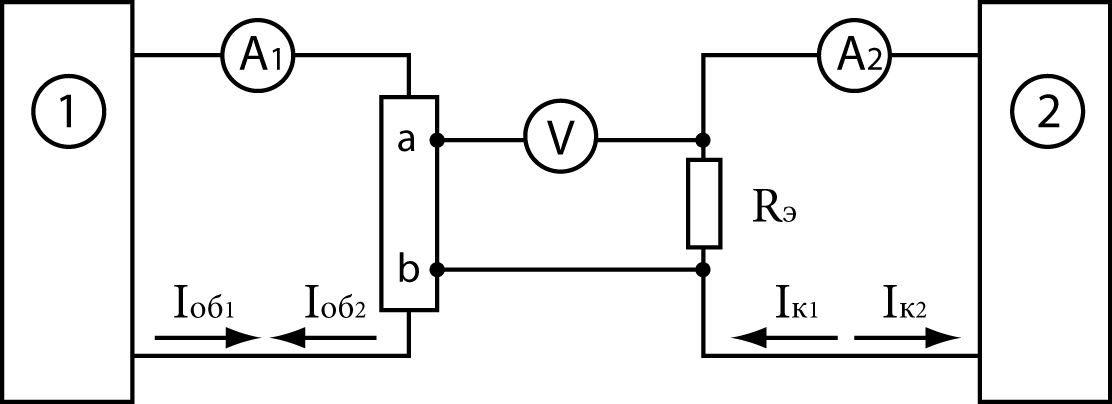
\includegraphics[width = .9\linewidth]{img/scheme.jpg}
	\caption{Электрическая схема для измерений удельной электропроводности методом компенсации}
	\label{fig:5.1}
\end{figure}

Регулируемый источник тока (1) задаёт ток образца $I_\text{об}$, измеряемый амперметром $A1$. Регулируемый источник тока
(2) задаёт ток компенсации $I_\text{к}$ через эталонный резистор $R_\text{э}$, величина этого тока измеряется
амперметром $А2$. Напряжение $U_{ab}$ между зондовыми электродами a и b сравнивается с напряжением компенсации $U_k$ на
эталонном резисторе $R_\text{э}$ при помощи индикатора компенсации V.

При проведении измерений нужно установить ток образца, затем, изменяя ток компенсации, добиться нулевых показаний
индикатора компенсации V. В этом случае напряжение $U_k$ на эталонном резисторе $R_\text{э}$ будет равно напряжению $U_{ab}$:
\begin{equation}
	U_{ab}=U_{k}=I_{k} R_{\text{э}} 
	\label{eq:5.1}
\end{equation}

В реальной ситуации между зондовыми электродами будут паразитные потенциалы, связанные, во-первых, с влиянием
переходного сопротивления на контактах «образец – подводящие провода», во-вторых, появлением термоЭДС на контактах
полупроводника с металлом при нагреве образца. Для того чтобы устранить влияние этих потенциалов, измерение тока
компенсации производится дважды. Получив первый отсчёт $I_{k1}$, изменяем направление тока через образец и через
эталонный резистор, опять добиваемся равенства напряжений $U_k$ и $U_{ab}$, снимаем второй отсчёт $I_{k2}$. Обратите
внимание, что полярность разности потенциалов между электродами a и b, вызванная протеканием тока через образец, как и
напряжение на $R_\text{э}$, сменились на противоположные, а паразитные потенциалы, зависящие от свойств контактов, и
термоЭДС, зависящая от температуры образца, остались прежние. Таким образом, среднеарифметическое значение 

$$I_k=\frac{I_{k1}+I_{k2}}{2}$$

будет содержать информацию только о полезной составляющей напряжения $U_{ab}$.

Величину падения напряжения $U_k$ легко подсчитать:
$$U_{k}=I_{k} R_{\text{э}}$$

Величину сопротивления участка образца расположенного между зондовыми электродами a и b ($R_{\text{об}}$) можно определить из равенства:
$$R_{\text{об}}=\frac{U_{k}}{I_{\text{об}}}=\frac{I_{k} R_{\text{э}}}{I_{\text{об}}}$$
Зная размеры образца: a - ширина (см), d - толщина (см), l - расстояние между электродами a и b (см), можно рассчитать удельное сопротивление образца:
$$\rho=\frac{d a}{l} R_{\text{об}} (\text{Oм} \text{ cм})$$

или обратную величину - удельную электропроводность: 
$$\sigma=1 / \rho\left(\text{Oм}^{-1} \text{cм}^{-1}\right)$$

\section{Схема экспериментальной установки}
Внешний вид установки можно увидеть на рис. \ref{fig:6.1}, а её схему – на рис. \ref{fig:6.2}. 

\begin{figure}[h!]
	\centering
	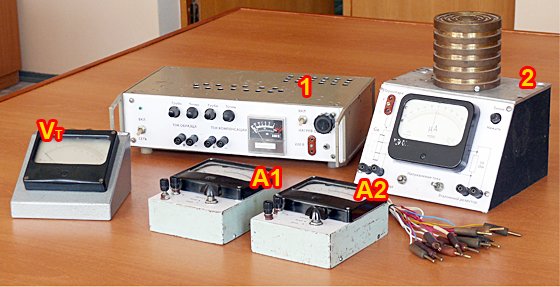
\includegraphics[width = .9\linewidth]{img/ust.jpg}
	\caption{Внешний вид установки}
	\label{fig:6.1}
\end{figure}

\begin{figure}[h!]
	\centering
	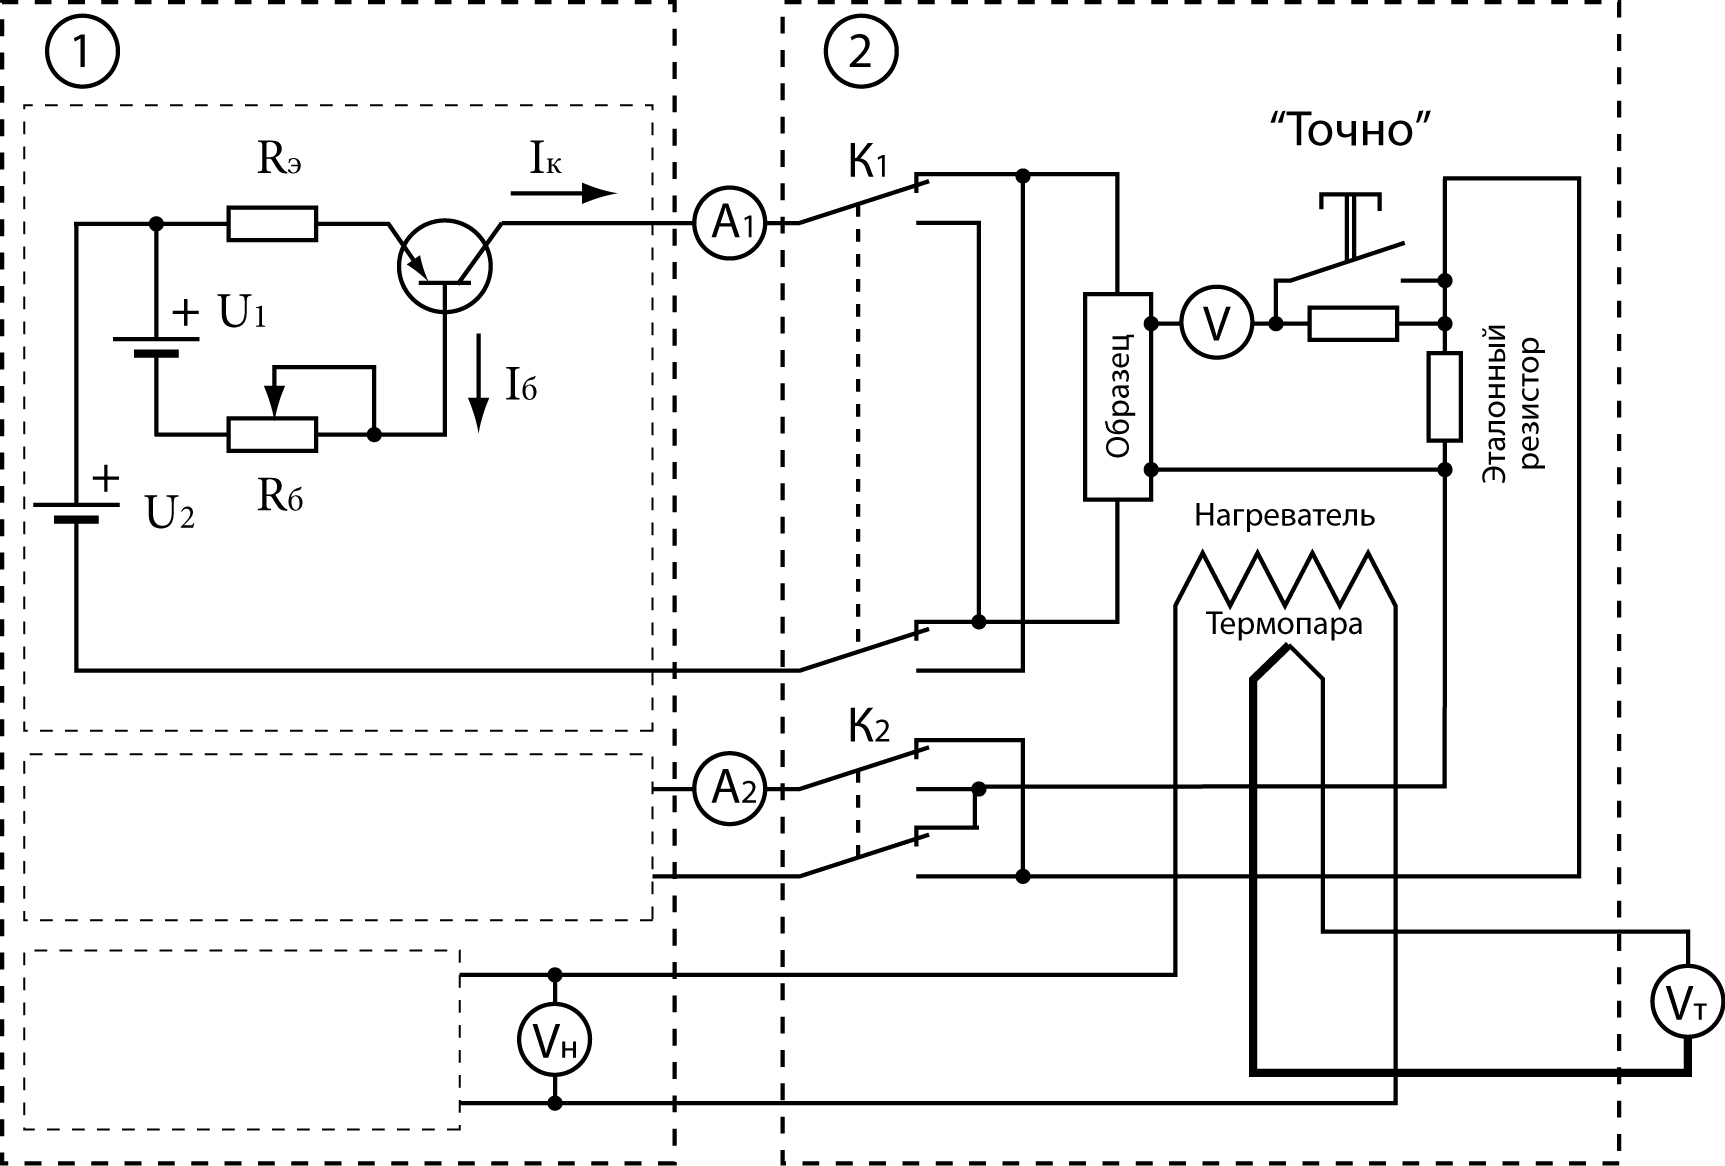
\includegraphics[width = .9\linewidth]{img/scheme-2.jpg}
	\caption{Схема установки}
	\label{fig:6.2}
\end{figure}

Блок питания (1) содержит в себе два регулируемых стабилизатора тока (для образца и эталонного резистора) и регулируемый
источник питания нагревателя образца, напряжение на выходе которого контролируется вольтметром $V_\text{н}$. На верхней
крышке измерительного блока (2) находится трубчатый керамический нагреватель, в котором размещён исследуемый образец и
термопара для измерения температуры. Нагреватель с образцом и термопарой закрыты защитным цилиндром. В корпусе
измерительного блока (2) располагается эталонный резистор Rэ, переключатели направления тока образца и компенсации К1 и
К2, индикатор компенсации V с переключателем чувствительности «Точно». Измерение токов образца и компенсации
производится миллиамперметрами А1 и А2 для измерения ЭДС термопары используется милливольтметр Vт, показания которого
пересчитываются в температуру по градуировочному графику (рис. \ref{fig:6.3}).

\begin{figure}[h!]
	\centering
	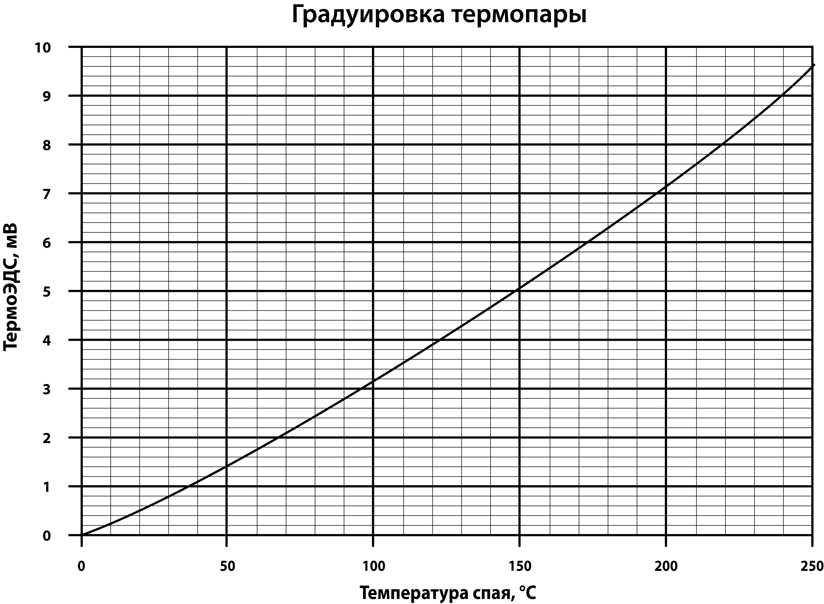
\includegraphics[width = .9\linewidth]{img/grad.jpg}
	\caption{График соответствия ЭДС термопары и температуры спая}
	\label{fig:6.3}
\end{figure}


\section*{Эксперимент}
\textbf{Оборудование}
\begin{enumerate}
	\item $R{\text{э}} = 10$ Ом.
	\item Образец $l = 7$ см, $d=1.4$ см, $a = 4$ см $x = 20$ см.
\end{enumerate}

Произвели измерение электропроводности образца при комнатной температуре. Установив ток образца 5-10 мА
добились нулевого отклонения индикатора. Аналогичное сделали, сменив направление тока.

Такие же измерения провели при различных температурах. Сняли температурную зависимость тока компенсации (для двух направлений тока при каждом
значении температуры $I_{k1},I_{k2}$).

Далее взяли среднее значение тока:
$$I_k=\frac{I_{k1}+I_{k2}}{2}$$

Рассчитали проводимость для каждой снятой точки по формуле:

$$\sigma = \frac{l}{ad} \frac{I_{\text{об}}}{ I_k ~ R_{\text{э}}}$$



\subsection*{Обработка результатов измерений}
Построили график полученной зависимости $ln~\sigma(\frac{10^3}{T})$ (Т – абсолютная температура в градусах К).

\begin{figure}[h!]
	\centering
	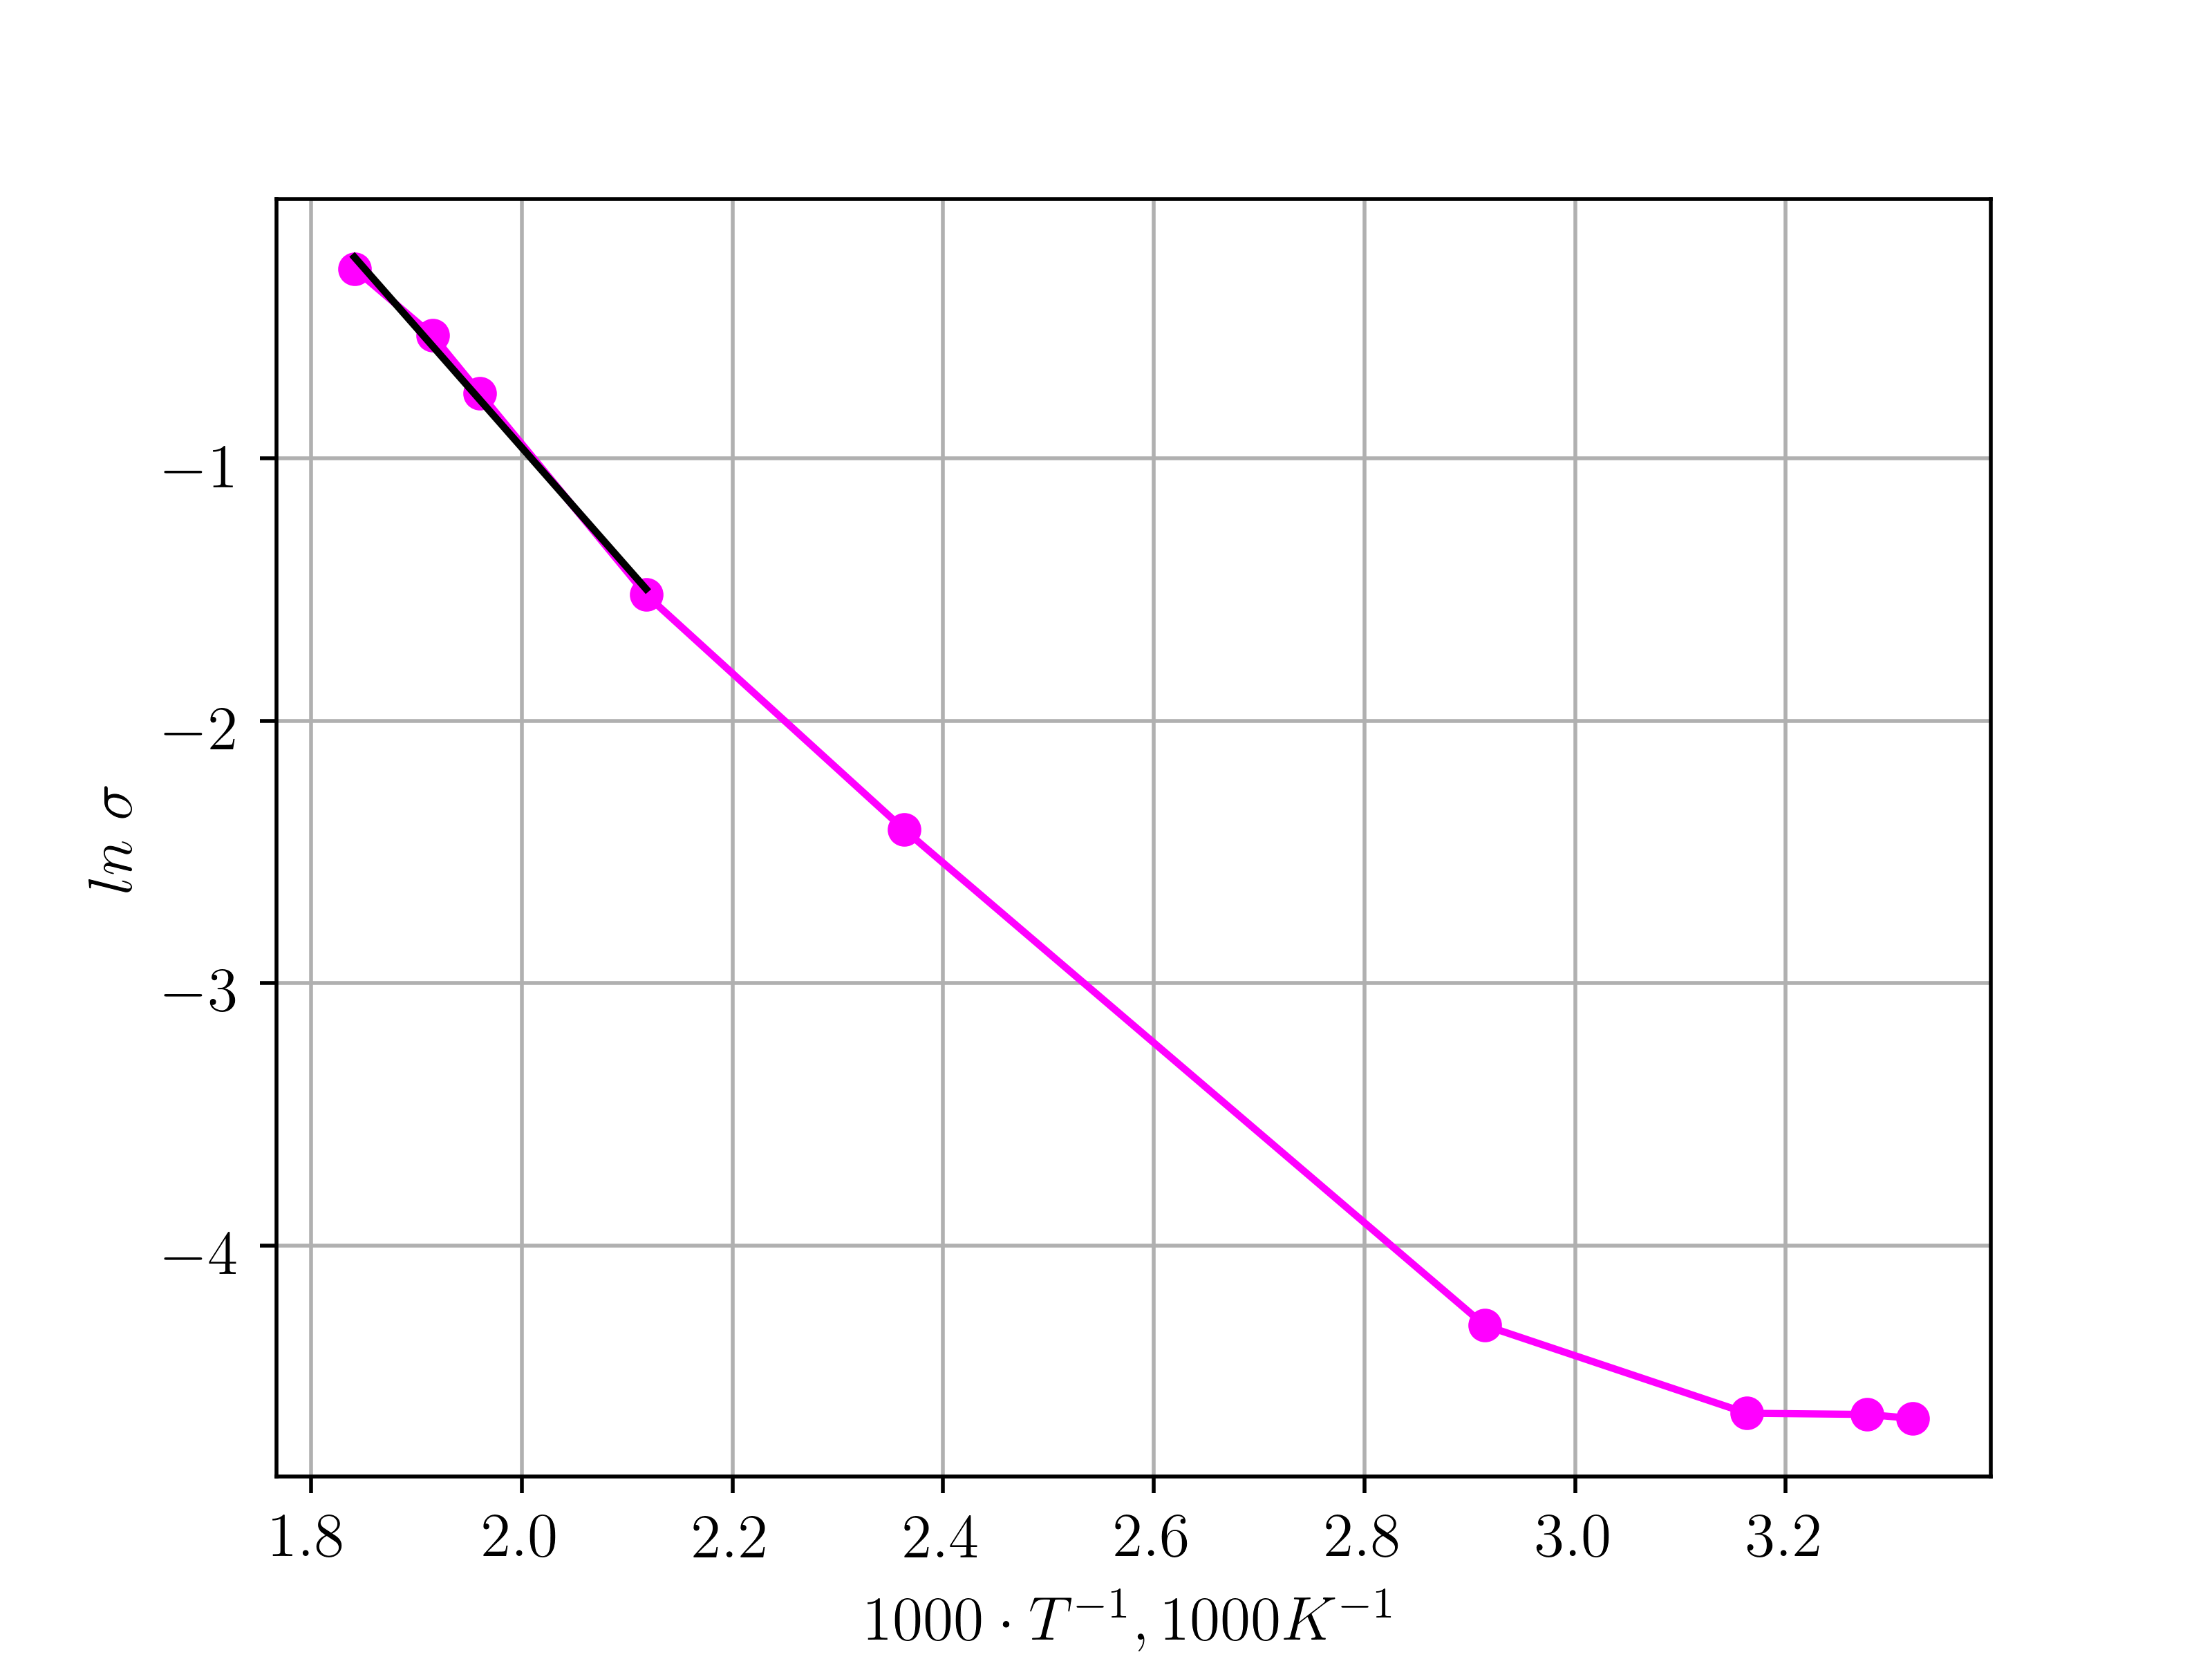
\includegraphics[width = .8\linewidth]{graphs/lns.png}
	\caption{}
	\label{fig:exp.1}
\end{figure}
Прологарифмировали выражение \eqref{eq:4.4} и нашли связь между угловым коэффициентом наклона кривой
$ln~\sigma(\frac{10^3}{T})$ и величиной $W_g$:

$$ ln(\sigma) = \underbrace{ln(\sigma_C)}_{const} - W_g /2 k_B T $$
$$ W_g = -1000 \cdot tan(\theta) \cdot 2 k_B $$
где $tan(\theta)$ - тангенс угла наклона графика $ln~\sigma(\frac{1}{T})$, $k_B \approx 8.62 \cdot 10^{-5}$ эВ/К -
постоянная Больцмана.

Определили угловой коэффициент наклона кривой в области высоких температур и рассчитали значение $W_g$:
$$tan(\theta) \approx -3.34 $$
$$ W_g \approx 0.58 \text{ эВ}$$ 

В области истощения примесей определить зависимость $\sigma = f(T)$, считая, что $\sigma \approx T^n$. Ее
можно найти, взяв на кривой две точки и воспользовавшись соотношением $\sigma_{I} / \sigma_{2}=\left(T_{I} /
T_{2}\right)^{n}$.

????


Определили (экстраполяцией по графику) величину $\sigma_c$, соответствующую
электропроводности вещества при $T \to \infty$.
$$\sigma_c = e^7 $$
выше бред ???????????


\end{document}
